\documentclass[1p]{elsarticle_modified}
%\bibliographystyle{elsarticle-num}

%\usepackage[colorlinks]{hyperref}
%\usepackage{abbrmath_seonhwa} %\Abb, \Ascr, \Acal ,\Abf, \Afrak
\usepackage{amsfonts}
\usepackage{amssymb}
\usepackage{amsmath}
\usepackage{amsthm}
\usepackage{scalefnt}
\usepackage{amsbsy}
\usepackage{kotex}
\usepackage{caption}
\usepackage{subfig}
\usepackage{color}
\usepackage{graphicx}
\usepackage{xcolor} %% white, black, red, green, blue, cyan, magenta, yellow
\usepackage{float}
\usepackage{setspace}
\usepackage{hyperref}

\usepackage{tikz}
\usetikzlibrary{arrows}

\usepackage{multirow}
\usepackage{array} % fixed length table
\usepackage{hhline}

%%%%%%%%%%%%%%%%%%%%%
\makeatletter
\renewcommand*\env@matrix[1][\arraystretch]{%
	\edef\arraystretch{#1}%
	\hskip -\arraycolsep
	\let\@ifnextchar\new@ifnextchar
	\array{*\c@MaxMatrixCols c}}
\makeatother %https://tex.stackexchange.com/questions/14071/how-can-i-increase-the-line-spacing-in-a-matrix
%%%%%%%%%%%%%%%

\usepackage[normalem]{ulem}

\newcommand{\msout}[1]{\ifmmode\text{\sout{\ensuremath{#1}}}\else\sout{#1}\fi}
%SOURCE: \msout is \stkout macro in https://tex.stackexchange.com/questions/20609/strikeout-in-math-mode

\newcommand{\cancel}[1]{
	\ifmmode
	{\color{red}\msout{#1}}
	\else
	{\color{red}\sout{#1}}
	\fi
}

\newcommand{\add}[1]{
	{\color{blue}\uwave{#1}}
}

\newcommand{\replace}[2]{
	\ifmmode
	{\color{red}\msout{#1}}{\color{blue}\uwave{#2}}
	\else
	{\color{red}\sout{#1}}{\color{blue}\uwave{#2}}
	\fi
}

\newcommand{\Sol}{\mathcal{S}} %segment
\newcommand{\D}{D} %diagram
\newcommand{\A}{\mathcal{A}} %arc


%%%%%%%%%%%%%%%%%%%%%%%%%%%%%5 test

\def\sl{\operatorname{\textup{SL}}(2,\Cbb)}
\def\psl{\operatorname{\textup{PSL}}(2,\Cbb)}
\def\quan{\mkern 1mu \triangleright \mkern 1mu}

\theoremstyle{definition}
\newtheorem{thm}{Theorem}[section]
\newtheorem{prop}[thm]{Proposition}
\newtheorem{lem}[thm]{Lemma}
\newtheorem{ques}[thm]{Question}
\newtheorem{cor}[thm]{Corollary}
\newtheorem{defn}[thm]{Definition}
\newtheorem{exam}[thm]{Example}
\newtheorem{rmk}[thm]{Remark}
\newtheorem{alg}[thm]{Algorithm}

\newcommand{\I}{\sqrt{-1}}
\begin{document}

%\begin{frontmatter}
%
%\title{Boundary parabolic representations of knots up to 8 crossings}
%
%%% Group authors per affiliation:
%\author{Yunhi Cho} 
%\address{Department of Mathematics, University of Seoul, Seoul, Korea}
%\ead{yhcho@uos.ac.kr}
%
%
%\author{Seonhwa Kim} %\fnref{s_kim}}
%\address{Center for Geometry and Physics, Institute for Basic Science, Pohang, 37673, Korea}
%\ead{ryeona17@ibs.re.kr}
%
%\author{Hyuk Kim}
%\address{Department of Mathematical Sciences, Seoul National University, Seoul 08826, Korea}
%\ead{hyukkim@snu.ac.kr}
%
%\author{Seokbeom Yoon}
%\address{Department of Mathematical Sciences, Seoul National University, Seoul, 08826,  Korea}
%\ead{sbyoon15@snu.ac.kr}
%
%\begin{abstract}
%We find all boundary parabolic representation of knots up to 8 crossings.
%
%\end{abstract}
%\begin{keyword}
%    \MSC[2010] 57M25 
%\end{keyword}
%
%\end{frontmatter}

%\linenumbers
%\tableofcontents
%
\newcommand\colored[1]{\textcolor{white}{\rule[-0.35ex]{0.8em}{1.4ex}}\kern-0.8em\color{red} #1}%
%\newcommand\colored[1]{\textcolor{white}{ #1}\kern-2.17ex	\textcolor{white}{ #1}\kern-1.81ex	\textcolor{white}{ #1}\kern-2.15ex\color{red}#1	}

{\Large $\underline{11n_{177}~(K11n_{177})}$}

\setlength{\tabcolsep}{10pt}
\renewcommand{\arraystretch}{1.6}
\vspace{1cm}\begin{tabular}{m{100pt}>{\centering\arraybackslash}m{274pt}}
\multirow{5}{120pt}{
	\centering
	\includegraphics[width=112pt]{../../../GIT/diagram.site/Diagrams/png/793_11n_177.png}\\
\ \ \ A knot diagram\footnotemark}&
\allowdisplaybreaks
\textbf{Linearized knot diagam} \\
\cline{2-2}
 &
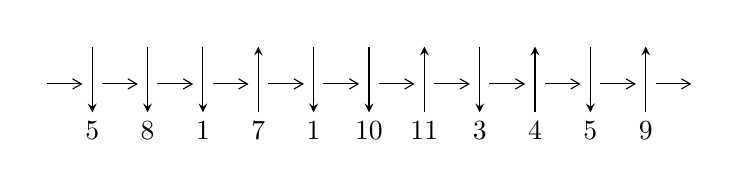
\begin{tikzpicture}[x=20pt, y=17pt]
	% nodes
	\node (C0) at (0, 0) {};
	\node (C1) at (1, 0) {};
	\node (C1U) at (1, +1) {};
	\node (C1D) at (1, -1) {5};

	\node (C2) at (2, 0) {};
	\node (C2U) at (2, +1) {};
	\node (C2D) at (2, -1) {8};

	\node (C3) at (3, 0) {};
	\node (C3U) at (3, +1) {};
	\node (C3D) at (3, -1) {1};

	\node (C4) at (4, 0) {};
	\node (C4U) at (4, +1) {};
	\node (C4D) at (4, -1) {7};

	\node (C5) at (5, 0) {};
	\node (C5U) at (5, +1) {};
	\node (C5D) at (5, -1) {1};

	\node (C6) at (6, 0) {};
	\node (C6U) at (6, +1) {};
	\node (C6D) at (6, -1) {10};

	\node (C7) at (7, 0) {};
	\node (C7U) at (7, +1) {};
	\node (C7D) at (7, -1) {11};

	\node (C8) at (8, 0) {};
	\node (C8U) at (8, +1) {};
	\node (C8D) at (8, -1) {3};

	\node (C9) at (9, 0) {};
	\node (C9U) at (9, +1) {};
	\node (C9D) at (9, -1) {4};

	\node (C10) at (10, 0) {};
	\node (C10U) at (10, +1) {};
	\node (C10D) at (10, -1) {5};

	\node (C11) at (11, 0) {};
	\node (C11U) at (11, +1) {};
	\node (C11D) at (11, -1) {9};
	\node (C12) at (12, 0) {};

	% arrows
	\draw[->,>={angle 60}]
	(C0) edge (C1) (C1) edge (C2) (C2) edge (C3) (C3) edge (C4) (C4) edge (C5) (C5) edge (C6) (C6) edge (C7) (C7) edge (C8) (C8) edge (C9) (C9) edge (C10) (C10) edge (C11) (C11) edge (C12) ;	\draw[->,>=stealth]
	(C1U) edge (C1D) (C2U) edge (C2D) (C3U) edge (C3D) (C4D) edge (C4U) (C5U) edge (C5D) (C6U) edge (C6D) (C7D) edge (C7U) (C8U) edge (C8D) (C9D) edge (C9U) (C10U) edge (C10D) (C11D) edge (C11U) ;
	\end{tikzpicture} \\
\hhline{~~} \\& 
\textbf{Solving Sequence} \\ \cline{2-2} 
 &
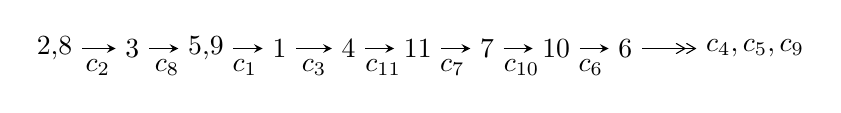
\begin{tikzpicture}[x=25pt, y=7pt]
	% node
	\node (A0) at (-1/8, 0) {2,8};
	\node (A1) at (1, 0) {3};
	\node (A2) at (33/16, 0) {5,9};
	\node (A3) at (25/8, 0) {1};
	\node (A4) at (33/8, 0) {4};
	\node (A5) at (41/8, 0) {11};
	\node (A6) at (49/8, 0) {7};
	\node (A7) at (57/8, 0) {10};
	\node (A8) at (65/8, 0) {6};
	\node (C1) at (1/2, -1) {$c_{2}$};
	\node (C2) at (3/2, -1) {$c_{8}$};
	\node (C3) at (21/8, -1) {$c_{1}$};
	\node (C4) at (29/8, -1) {$c_{3}$};
	\node (C5) at (37/8, -1) {$c_{11}$};
	\node (C6) at (45/8, -1) {$c_{7}$};
	\node (C7) at (53/8, -1) {$c_{10}$};
	\node (C8) at (61/8, -1) {$c_{6}$};
	\node (A9) at (10, 0) {$c_{4},c_{5},c_{9}$};

	% edge
	\draw[->,>=stealth]	
	(A0) edge (A1) (A1) edge (A2) (A2) edge (A3) (A3) edge (A4) (A4) edge (A5) (A5) edge (A6) (A6) edge (A7) (A7) edge (A8) ;
	\draw[->>,>={angle 60}]	
	(A8) edge (A9);
\end{tikzpicture} \\ 

\end{tabular} \\

\footnotetext{
The image of knot diagram is generated by the software ``\textbf{Draw programme}" developed by Andrew Bartholomew(\url{http://www.layer8.co.uk/maths/draw/index.htm\#Running-draw}), where we modified some parts for our purpose(\url{https://github.com/CATsTAILs/LinksPainter}).
}\phantom \\ \newline 
\centering \textbf{Ideals for irreducible components\footnotemark of $X_{\text{par}}$} 
 
\begin{align*}
I^u_{1}&=\langle 
-3.24572\times10^{142} u^{60}+1.72689\times10^{142} u^{59}+\cdots+4.07698\times10^{142} b-1.22998\times10^{145},\\
\phantom{I^u_{1}}&\phantom{= \langle  }-2.97918\times10^{145} u^{60}+1.11595\times10^{145} u^{59}+\cdots+8.60243\times10^{144} a-1.02025\times10^{148},\\
\phantom{I^u_{1}}&\phantom{= \langle  }u^{61}- u^{60}+\cdots+1440 u-211\rangle \\
I^u_{2}&=\langle 
-191 u^{19}-54 u^{18}+\cdots+871 b-1760,\;-5462 u^{19}+3472 u^{18}+\cdots+871 a-3488,\\
\phantom{I^u_{2}}&\phantom{= \langle  }u^{20}-10 u^{18}+\cdots-3 u+1\rangle \\
\\
\end{align*}
\raggedright * 2 irreducible components of $\dim_{\mathbb{C}}=0$, with total 81 representations.\\
\footnotetext{All coefficients of polynomials are rational numbers. But the coefficients are sometimes approximated in decimal forms when there is not enough margin.}
\newpage
\renewcommand{\arraystretch}{1}
\centering \section*{I. $I^u_{1}= \langle -3.25\times10^{142} u^{60}+1.73\times10^{142} u^{59}+\cdots+4.08\times10^{142} b-1.23\times10^{145},\;-2.98\times10^{145} u^{60}+1.12\times10^{145} u^{59}+\cdots+8.60\times10^{144} a-1.02\times10^{148},\;u^{61}- u^{60}+\cdots+1440 u-211 \rangle$}
\flushleft \textbf{(i) Arc colorings}\\
\begin{tabular}{m{7pt} m{180pt} m{7pt} m{180pt} }
\flushright $a_{2}=$&$\begin{pmatrix}1\\0\end{pmatrix}$ \\
\flushright $a_{8}=$&$\begin{pmatrix}0\\u\end{pmatrix}$ \\
\flushright $a_{3}=$&$\begin{pmatrix}1\\u^2\end{pmatrix}$ \\
\flushright $a_{5}=$&$\begin{pmatrix}3.46318 u^{60}-1.29725 u^{59}+\cdots-6140.42 u+1186.01\\0.796110 u^{60}-0.423570 u^{59}+\cdots-1559.98 u+301.690\end{pmatrix}$ \\
\flushright $a_{9}=$&$\begin{pmatrix}- u\\- u^3+u\end{pmatrix}$ \\
\flushright $a_{1}=$&$\begin{pmatrix}1.29224 u^{60}-0.448881 u^{59}+\cdots-2255.76 u+429.617\\1.27366 u^{60}-0.370816 u^{59}+\cdots-2085.03 u+390.903\end{pmatrix}$ \\
\flushright $a_{4}=$&$\begin{pmatrix}1.28221 u^{60}-0.453127 u^{59}+\cdots-2204.36 u+413.438\\-0.635387 u^{60}+0.249195 u^{59}+\cdots+1132.30 u-216.875\end{pmatrix}$ \\
\flushright $a_{11}=$&$\begin{pmatrix}0.388456 u^{60}-0.195779 u^{59}+\cdots-775.545 u+151.289\\1.67899 u^{60}-0.538031 u^{59}+\cdots-2818.97 u+531.938\end{pmatrix}$ \\
\flushright $a_{7}=$&$\begin{pmatrix}-0.630060 u^{60}+0.197657 u^{59}+\cdots+1058.49 u-208.443\\-2.03043 u^{60}+0.716573 u^{59}+\cdots+3492.84 u-661.096\end{pmatrix}$ \\
\flushright $a_{10}=$&$\begin{pmatrix}-0.747989 u^{60}+0.276535 u^{59}+\cdots+1286.06 u-236.612\\0.433328 u^{60}-0.123845 u^{59}+\cdots-717.355 u+135.073\end{pmatrix}$ \\
\flushright $a_{6}=$&$\begin{pmatrix}-1.16771 u^{60}+0.323667 u^{59}+\cdots+1929.57 u-371.367\\-1.29217 u^{60}+0.498917 u^{59}+\cdots+2268.85 u-430.204\end{pmatrix}$\\ \flushright $a_{6}=$&$\begin{pmatrix}-1.16771 u^{60}+0.323667 u^{59}+\cdots+1929.57 u-371.367\\-1.29217 u^{60}+0.498917 u^{59}+\cdots+2268.85 u-430.204\end{pmatrix}$\\&\end{tabular}
\flushleft \textbf{(ii) Obstruction class $= -1$}\\~\\
\flushleft \textbf{(iii) Cusp Shapes $= -7.66374 u^{60}+2.83409 u^{59}+\cdots+13662.1 u-2642.77$}\\~\\
\newpage\renewcommand{\arraystretch}{1}
\flushleft \textbf{(iv) u-Polynomials at the component}\newline \\
\begin{tabular}{m{50pt}|m{274pt}}
Crossings & \hspace{64pt}u-Polynomials at each crossing \\
\hline $$\begin{aligned}c_{1},c_{5}\end{aligned}$$&$\begin{aligned}
&u^{61}+2 u^{60}+\cdots-25 u+1
\end{aligned}$\\
\hline $$\begin{aligned}c_{2},c_{8}\end{aligned}$$&$\begin{aligned}
&u^{61}- u^{60}+\cdots+1440 u-211
\end{aligned}$\\
\hline $$\begin{aligned}c_{3}\end{aligned}$$&$\begin{aligned}
&u^{61}-4 u^{60}+\cdots-957 u+121
\end{aligned}$\\
\hline $$\begin{aligned}c_{4}\end{aligned}$$&$\begin{aligned}
&u^{61}+6 u^{60}+\cdots+22 u+1
\end{aligned}$\\
\hline $$\begin{aligned}c_{6}\end{aligned}$$&$\begin{aligned}
&u^{61}+4 u^{60}+\cdots+6790 u-2531
\end{aligned}$\\
\hline $$\begin{aligned}c_{7}\end{aligned}$$&$\begin{aligned}
&u^{61}+u^{60}+\cdots-9850 u-2333
\end{aligned}$\\
\hline $$\begin{aligned}c_{9}\end{aligned}$$&$\begin{aligned}
&u^{61}+2 u^{60}+\cdots+529 u+41
\end{aligned}$\\
\hline $$\begin{aligned}c_{10}\end{aligned}$$&$\begin{aligned}
&u^{61}-10 u^{59}+\cdots-62973 u+14123
\end{aligned}$\\
\hline $$\begin{aligned}c_{11}\end{aligned}$$&$\begin{aligned}
&u^{61}-4 u^{60}+\cdots+6 u+1
\end{aligned}$\\
\hline
\end{tabular}\\~\\
\newpage\renewcommand{\arraystretch}{1}
\flushleft \textbf{(v) Riley Polynomials at the component}\newline \\
\begin{tabular}{m{50pt}|m{274pt}}
Crossings & \hspace{64pt}Riley Polynomials at each crossing \\
\hline $$\begin{aligned}c_{1},c_{5}\end{aligned}$$&$\begin{aligned}
&y^{61}-54 y^{60}+\cdots+111 y-1
\end{aligned}$\\
\hline $$\begin{aligned}c_{2},c_{8}\end{aligned}$$&$\begin{aligned}
&y^{61}-57 y^{60}+\cdots+631204 y-44521
\end{aligned}$\\
\hline $$\begin{aligned}c_{3}\end{aligned}$$&$\begin{aligned}
&y^{61}-28 y^{60}+\cdots+684255 y-14641
\end{aligned}$\\
\hline $$\begin{aligned}c_{4}\end{aligned}$$&$\begin{aligned}
&y^{61}-16 y^{60}+\cdots+364 y-1
\end{aligned}$\\
\hline $$\begin{aligned}c_{6}\end{aligned}$$&$\begin{aligned}
&y^{61}-14 y^{60}+\cdots+234688910 y-6405961
\end{aligned}$\\
\hline $$\begin{aligned}c_{7}\end{aligned}$$&$\begin{aligned}
&y^{61}+23 y^{60}+\cdots+27116488 y-5442889
\end{aligned}$\\
\hline $$\begin{aligned}c_{9}\end{aligned}$$&$\begin{aligned}
&y^{61}+52 y^{59}+\cdots-12653 y-1681
\end{aligned}$\\
\hline $$\begin{aligned}c_{10}\end{aligned}$$&$\begin{aligned}
&y^{61}-20 y^{60}+\cdots+4161767199 y-199459129
\end{aligned}$\\
\hline $$\begin{aligned}c_{11}\end{aligned}$$&$\begin{aligned}
&y^{61}-8 y^{60}+\cdots+12 y-1
\end{aligned}$\\
\hline
\end{tabular}\\~\\
\newpage\flushleft \textbf{(vi) Complex Volumes and Cusp Shapes}
$$\begin{array}{c|c|c}  
\text{Solutions to }I^u_{1}& \I (\text{vol} + \sqrt{-1}CS) & \text{Cusp shape}\\
 \hline 
\begin{aligned}
u &= -0.976776 + 0.468629 I \\
a &= -0.15466 - 1.57760 I \\
b &= -1.360820 + 0.112274 I\end{aligned}
 & -3.79970 + 5.99586 I & \phantom{-0.000000 } 0 \\ \hline\begin{aligned}
u &= -0.976776 - 0.468629 I \\
a &= -0.15466 + 1.57760 I \\
b &= -1.360820 - 0.112274 I\end{aligned}
 & -3.79970 - 5.99586 I & \phantom{-0.000000 } 0 \\ \hline\begin{aligned}
u &= -0.524227 + 0.745772 I \\
a &= -0.531624 + 0.534873 I \\
b &= \phantom{-}1.50782 - 0.08700 I\end{aligned}
 & -2.50680 - 1.31837 I & \phantom{-0.000000 } 0 \\ \hline\begin{aligned}
u &= -0.524227 - 0.745772 I \\
a &= -0.531624 - 0.534873 I \\
b &= \phantom{-}1.50782 + 0.08700 I\end{aligned}
 & -2.50680 + 1.31837 I & \phantom{-0.000000 } 0 \\ \hline\begin{aligned}
u &= \phantom{-}0.678087 + 0.569708 I \\
a &= \phantom{-}0.116142 - 0.826864 I \\
b &= -0.368363 + 0.027145 I\end{aligned}
 & \phantom{-}1.88623 - 2.18277 I & \phantom{-0.000000 } 0 \\ \hline\begin{aligned}
u &= \phantom{-}0.678087 - 0.569708 I \\
a &= \phantom{-}0.116142 + 0.826864 I \\
b &= -0.368363 - 0.027145 I\end{aligned}
 & \phantom{-}1.88623 + 2.18277 I & \phantom{-0.000000 } 0 \\ \hline\begin{aligned}
u &= \phantom{-}0.868659 + 0.085320 I \\
a &= \phantom{-}0.448202 + 1.164690 I \\
b &= -0.064748 + 1.346320 I\end{aligned}
 & \phantom{-}4.49837 - 0.35042 I & \phantom{-}4.30932 - 5.56885 I \\ \hline\begin{aligned}
u &= \phantom{-}0.868659 - 0.085320 I \\
a &= \phantom{-}0.448202 - 1.164690 I \\
b &= -0.064748 - 1.346320 I\end{aligned}
 & \phantom{-}4.49837 + 0.35042 I & \phantom{-}4.30932 + 5.56885 I \\ \hline\begin{aligned}
u &= \phantom{-}1.127820 + 0.013378 I \\
a &= \phantom{-}0.848633 - 0.329495 I \\
b &= \phantom{-}0.484117 + 0.888170 I\end{aligned}
 & \phantom{-}0.28694 - 2.95538 I & \phantom{-0.000000 } 0 \\ \hline\begin{aligned}
u &= \phantom{-}1.127820 - 0.013378 I \\
a &= \phantom{-}0.848633 + 0.329495 I \\
b &= \phantom{-}0.484117 - 0.888170 I\end{aligned}
 & \phantom{-}0.28694 + 2.95538 I & \phantom{-0.000000 } 0\\
 \hline 
 \end{array}$$\newpage$$\begin{array}{c|c|c}  
\text{Solutions to }I^u_{1}& \I (\text{vol} + \sqrt{-1}CS) & \text{Cusp shape}\\
 \hline 
\begin{aligned}
u &= -0.827402 + 0.215446 I \\
a &= \phantom{-}0.369344 + 0.142430 I \\
b &= \phantom{-}0.572552 - 0.128270 I\end{aligned}
 & -1.311000 + 0.288972 I & -7.97577 + 0. I\phantom{ +0.000000I} \\ \hline\begin{aligned}
u &= -0.827402 - 0.215446 I \\
a &= \phantom{-}0.369344 - 0.142430 I \\
b &= \phantom{-}0.572552 + 0.128270 I\end{aligned}
 & -1.311000 - 0.288972 I & -7.97577 + 0. I\phantom{ +0.000000I} \\ \hline\begin{aligned}
u &= \phantom{-}0.430791 + 0.712040 I \\
a &= \phantom{-}0.206810 - 0.287330 I \\
b &= -0.162616 - 0.032660 I\end{aligned}
 & \phantom{-}2.67011 + 1.18908 I & -3.00000 + 2.70122 I \\ \hline\begin{aligned}
u &= \phantom{-}0.430791 - 0.712040 I \\
a &= \phantom{-}0.206810 + 0.287330 I \\
b &= -0.162616 + 0.032660 I\end{aligned}
 & \phantom{-}2.67011 - 1.18908 I & -3.00000 - 2.70122 I \\ \hline\begin{aligned}
u &= \phantom{-}1.101970 + 0.412324 I \\
a &= -0.694898 - 0.236565 I \\
b &= \phantom{-}0.101449 + 0.170923 I\end{aligned}
 & -2.45305 - 5.61811 I & \phantom{-0.000000 } 0 \\ \hline\begin{aligned}
u &= \phantom{-}1.101970 - 0.412324 I \\
a &= -0.694898 + 0.236565 I \\
b &= \phantom{-}0.101449 - 0.170923 I\end{aligned}
 & -2.45305 + 5.61811 I & \phantom{-0.000000 } 0 \\ \hline\begin{aligned}
u &= \phantom{-}0.725508 + 0.953905 I \\
a &= \phantom{-}0.42999 - 1.48215 I \\
b &= \phantom{-}0.16870 + 1.40882 I\end{aligned}
 & \phantom{-}4.00502 - 3.50717 I & \phantom{-0.000000 } 0 \\ \hline\begin{aligned}
u &= \phantom{-}0.725508 - 0.953905 I \\
a &= \phantom{-}0.42999 + 1.48215 I \\
b &= \phantom{-}0.16870 - 1.40882 I\end{aligned}
 & \phantom{-}4.00502 + 3.50717 I & \phantom{-0.000000 } 0 \\ \hline\begin{aligned}
u &= -1.21359\phantom{ +0.000000I} \\
a &= -2.56444\phantom{ +0.000000I} \\
b &= -1.62558\phantom{ +0.000000I}\end{aligned}
 & -4.17679\phantom{ +0.000000I} & \phantom{-0.000000 } 0 \\ \hline\begin{aligned}
u &= \phantom{-}1.072200 + 0.597671 I \\
a &= \phantom{-}0.029187 - 0.276448 I \\
b &= -0.0817486 + 0.0591173 I\end{aligned}
 & \phantom{-}0.79598 - 6.19961 I & \phantom{-0.000000 } 0\\
 \hline 
 \end{array}$$\newpage$$\begin{array}{c|c|c}  
\text{Solutions to }I^u_{1}& \I (\text{vol} + \sqrt{-1}CS) & \text{Cusp shape}\\
 \hline 
\begin{aligned}
u &= \phantom{-}1.072200 - 0.597671 I \\
a &= \phantom{-}0.029187 + 0.276448 I \\
b &= -0.0817486 - 0.0591173 I\end{aligned}
 & \phantom{-}0.79598 + 6.19961 I & \phantom{-0.000000 } 0 \\ \hline\begin{aligned}
u &= -0.325827 + 0.608474 I \\
a &= \phantom{-}0.939738 + 0.068849 I \\
b &= \phantom{-}1.142560 + 0.067073 I\end{aligned}
 & -1.23241 - 1.81263 I & \phantom{-}4.83572 + 3.41464 I \\ \hline\begin{aligned}
u &= -0.325827 - 0.608474 I \\
a &= \phantom{-}0.939738 - 0.068849 I \\
b &= \phantom{-}1.142560 - 0.067073 I\end{aligned}
 & -1.23241 + 1.81263 I & \phantom{-}4.83572 - 3.41464 I \\ \hline\begin{aligned}
u &= -1.296100 + 0.257994 I \\
a &= -1.94339 - 0.43070 I \\
b &= -1.63146 - 0.09947 I\end{aligned}
 & -4.62267 + 5.03624 I & \phantom{-0.000000 } 0 \\ \hline\begin{aligned}
u &= -1.296100 - 0.257994 I \\
a &= -1.94339 + 0.43070 I \\
b &= -1.63146 + 0.09947 I\end{aligned}
 & -4.62267 - 5.03624 I & \phantom{-0.000000 } 0 \\ \hline\begin{aligned}
u &= -1.318920 + 0.232232 I \\
a &= \phantom{-}0.289966 - 0.419451 I \\
b &= \phantom{-}0.121333 - 1.299240 I\end{aligned}
 & -4.69632 + 0.83070 I & \phantom{-0.000000 } 0 \\ \hline\begin{aligned}
u &= -1.318920 - 0.232232 I \\
a &= \phantom{-}0.289966 + 0.419451 I \\
b &= \phantom{-}0.121333 + 1.299240 I\end{aligned}
 & -4.69632 - 0.83070 I & \phantom{-0.000000 } 0 \\ \hline\begin{aligned}
u &= -1.355280 + 0.007498 I \\
a &= \phantom{-}2.05034 + 0.41832 I \\
b &= \phantom{-}1.57888 - 0.10960 I\end{aligned}
 & -8.02679 - 3.97936 I & \phantom{-0.000000 } 0 \\ \hline\begin{aligned}
u &= -1.355280 - 0.007498 I \\
a &= \phantom{-}2.05034 - 0.41832 I \\
b &= \phantom{-}1.57888 + 0.10960 I\end{aligned}
 & -8.02679 + 3.97936 I & \phantom{-0.000000 } 0 \\ \hline\begin{aligned}
u &= \phantom{-}0.641002 + 0.014713 I \\
a &= \phantom{-}0.47554 - 2.09406 I \\
b &= -0.425124 - 0.689408 I\end{aligned}
 & \phantom{-}2.15550 - 2.60300 I & -3.71097 + 4.89250 I\\
 \hline 
 \end{array}$$\newpage$$\begin{array}{c|c|c}  
\text{Solutions to }I^u_{1}& \I (\text{vol} + \sqrt{-1}CS) & \text{Cusp shape}\\
 \hline 
\begin{aligned}
u &= \phantom{-}0.641002 - 0.014713 I \\
a &= \phantom{-}0.47554 + 2.09406 I \\
b &= -0.425124 + 0.689408 I\end{aligned}
 & \phantom{-}2.15550 + 2.60300 I & -3.71097 - 4.89250 I \\ \hline\begin{aligned}
u &= \phantom{-}1.380460 + 0.006140 I \\
a &= -0.106176 - 1.042480 I \\
b &= -0.152247 + 0.537690 I\end{aligned}
 & \phantom{-}0.20782 - 3.93388 I & \phantom{-0.000000 } 0 \\ \hline\begin{aligned}
u &= \phantom{-}1.380460 - 0.006140 I \\
a &= -0.106176 + 1.042480 I \\
b &= -0.152247 - 0.537690 I\end{aligned}
 & \phantom{-}0.20782 + 3.93388 I & \phantom{-0.000000 } 0 \\ \hline\begin{aligned}
u &= \phantom{-}1.371230 + 0.218015 I \\
a &= \phantom{-}1.64543 - 0.22255 I \\
b &= \phantom{-}1.62447 + 0.87740 I\end{aligned}
 & -8.65446 - 7.29554 I & \phantom{-0.000000 } 0 \\ \hline\begin{aligned}
u &= \phantom{-}1.371230 - 0.218015 I \\
a &= \phantom{-}1.64543 + 0.22255 I \\
b &= \phantom{-}1.62447 - 0.87740 I\end{aligned}
 & -8.65446 + 7.29554 I & \phantom{-0.000000 } 0 \\ \hline\begin{aligned}
u &= \phantom{-}0.256892 + 0.520615 I \\
a &= \phantom{-}0.962604 + 0.557526 I \\
b &= -0.018225 - 0.428123 I\end{aligned}
 & -0.17125 + 1.80764 I & -1.37492 - 3.40193 I \\ \hline\begin{aligned}
u &= \phantom{-}0.256892 - 0.520615 I \\
a &= \phantom{-}0.962604 - 0.557526 I \\
b &= -0.018225 + 0.428123 I\end{aligned}
 & -0.17125 - 1.80764 I & -1.37492 + 3.40193 I \\ \hline\begin{aligned}
u &= -0.27863 + 1.40849 I \\
a &= -0.172968 - 0.248864 I \\
b &= -1.61867 + 0.35060 I\end{aligned}
 & -2.68997 + 9.29142 I & \phantom{-0.000000 } 0 \\ \hline\begin{aligned}
u &= -0.27863 - 1.40849 I \\
a &= -0.172968 + 0.248864 I \\
b &= -1.61867 - 0.35060 I\end{aligned}
 & -2.68997 - 9.29142 I & \phantom{-0.000000 } 0 \\ \hline\begin{aligned}
u &= -0.16045 + 1.43558 I \\
a &= \phantom{-}0.287870 + 0.352022 I \\
b &= \phantom{-}1.44542 - 0.44164 I\end{aligned}
 & -4.00110 + 1.61857 I & \phantom{-0.000000 } 0\\
 \hline 
 \end{array}$$\newpage$$\begin{array}{c|c|c}  
\text{Solutions to }I^u_{1}& \I (\text{vol} + \sqrt{-1}CS) & \text{Cusp shape}\\
 \hline 
\begin{aligned}
u &= -0.16045 - 1.43558 I \\
a &= \phantom{-}0.287870 - 0.352022 I \\
b &= \phantom{-}1.44542 + 0.44164 I\end{aligned}
 & -4.00110 - 1.61857 I & \phantom{-0.000000 } 0 \\ \hline\begin{aligned}
u &= -0.550059\phantom{ +0.000000I} \\
a &= -0.221675\phantom{ +0.000000I} \\
b &= \phantom{-}1.15486\phantom{ +0.000000I}\end{aligned}
 & -1.86682\phantom{ +0.000000I} & -10.5560\phantom{ +0.000000I} \\ \hline\begin{aligned}
u &= \phantom{-}1.44832 + 0.14867 I \\
a &= -1.62095 + 0.20059 I \\
b &= -1.65615 - 0.59781 I\end{aligned}
 & -9.14900 - 1.39395 I & \phantom{-0.000000 } 0 \\ \hline\begin{aligned}
u &= \phantom{-}1.44832 - 0.14867 I \\
a &= -1.62095 - 0.20059 I \\
b &= -1.65615 + 0.59781 I\end{aligned}
 & -9.14900 + 1.39395 I & \phantom{-0.000000 } 0 \\ \hline\begin{aligned}
u &= -1.48243 + 0.25068 I \\
a &= -0.223696 + 0.544024 I \\
b &= \phantom{-}0.07169 + 1.80725 I\end{aligned}
 & -3.01562 + 7.11329 I & \phantom{-0.000000 } 0 \\ \hline\begin{aligned}
u &= -1.48243 - 0.25068 I \\
a &= -0.223696 - 0.544024 I \\
b &= \phantom{-}0.07169 - 1.80725 I\end{aligned}
 & -3.01562 - 7.11329 I & \phantom{-0.000000 } 0 \\ \hline\begin{aligned}
u &= -1.53749 + 0.15211 I \\
a &= \phantom{-}1.50614 + 0.01272 I \\
b &= \phantom{-}1.68160 + 0.13329 I\end{aligned}
 & -5.39490 + 4.53513 I & \phantom{-0.000000 } 0 \\ \hline\begin{aligned}
u &= -1.53749 - 0.15211 I \\
a &= \phantom{-}1.50614 - 0.01272 I \\
b &= \phantom{-}1.68160 - 0.13329 I\end{aligned}
 & -5.39490 - 4.53513 I & \phantom{-0.000000 } 0 \\ \hline\begin{aligned}
u &= \phantom{-}0.406916 + 0.168439 I \\
a &= -1.25472 - 5.36486 I \\
b &= \phantom{-}0.074077 + 0.800622 I\end{aligned}
 & \phantom{-}3.77024 - 4.53103 I & \phantom{-}8.22458 + 6.69536 I \\ \hline\begin{aligned}
u &= \phantom{-}0.406916 - 0.168439 I \\
a &= -1.25472 + 5.36486 I \\
b &= \phantom{-}0.074077 - 0.800622 I\end{aligned}
 & \phantom{-}3.77024 + 4.53103 I & \phantom{-}8.22458 - 6.69536 I\\
 \hline 
 \end{array}$$\newpage$$\begin{array}{c|c|c}  
\text{Solutions to }I^u_{1}& \I (\text{vol} + \sqrt{-1}CS) & \text{Cusp shape}\\
 \hline 
\begin{aligned}
u &= \phantom{-}1.58071\phantom{ +0.000000I} \\
a &= -1.63264\phantom{ +0.000000I} \\
b &= -1.63455\phantom{ +0.000000I}\end{aligned}
 & -8.81824\phantom{ +0.000000I} & \phantom{-0.000000 } 0 \\ \hline\begin{aligned}
u &= \phantom{-}1.48930 + 0.55441 I \\
a &= -1.50676 + 0.66570 I \\
b &= -1.57377 - 0.77902 I\end{aligned}
 & -9.28034 - 8.26953 I & \phantom{-0.000000 } 0 \\ \hline\begin{aligned}
u &= \phantom{-}1.48930 - 0.55441 I \\
a &= -1.50676 - 0.66570 I \\
b &= -1.57377 + 0.77902 I\end{aligned}
 & -9.28034 + 8.26953 I & \phantom{-0.000000 } 0 \\ \hline\begin{aligned}
u &= -0.112871 + 0.355025 I \\
a &= \phantom{-}2.02427 - 0.38887 I \\
b &= -1.322340 + 0.325664 I\end{aligned}
 & -3.79837 + 4.86090 I & -6.23298 - 3.29979 I \\ \hline\begin{aligned}
u &= -0.112871 - 0.355025 I \\
a &= \phantom{-}2.02427 + 0.38887 I \\
b &= -1.322340 - 0.325664 I\end{aligned}
 & -3.79837 - 4.86090 I & -6.23298 + 3.29979 I \\ \hline\begin{aligned}
u &= \phantom{-}1.53961 + 0.56058 I \\
a &= \phantom{-}1.46289 - 0.60290 I \\
b &= \phantom{-}1.72297 + 0.74156 I\end{aligned}
 & -8.3594 - 16.0917 I & \phantom{-0.000000 } 0 \\ \hline\begin{aligned}
u &= \phantom{-}1.53961 - 0.56058 I \\
a &= \phantom{-}1.46289 + 0.60290 I \\
b &= \phantom{-}1.72297 - 0.74156 I\end{aligned}
 & -8.3594 + 16.0917 I & \phantom{-0.000000 } 0 \\ \hline\begin{aligned}
u &= -1.56552 + 0.57554 I \\
a &= -1.222210 - 0.542653 I \\
b &= -1.62521 + 0.02936 I\end{aligned}
 & -9.08401 + 5.81465 I & \phantom{-0.000000 } 0 \\ \hline\begin{aligned}
u &= -1.56552 - 0.57554 I \\
a &= -1.222210 + 0.542653 I \\
b &= -1.62521 - 0.02936 I\end{aligned}
 & -9.08401 - 5.81465 I & \phantom{-0.000000 } 0 \\ \hline\begin{aligned}
u &= -2.18540 + 0.57081 I \\
a &= \phantom{-}0.915634 + 0.234163 I \\
b &= \phantom{-}1.81648 - 0.11524 I\end{aligned}
 & -6.95721 + 0.21792 I & \phantom{-0.000000 } 0\\
 \hline 
 \end{array}$$\newpage$$\begin{array}{c|c|c}  
\text{Solutions to }I^u_{1}& \I (\text{vol} + \sqrt{-1}CS) & \text{Cusp shape}\\
 \hline 
\begin{aligned}
u &= -2.18540 - 0.57081 I \\
a &= \phantom{-}0.915634 - 0.234163 I \\
b &= \phantom{-}1.81648 + 0.11524 I\end{aligned}
 & -6.95721 - 0.21792 I & \phantom{-0.000000 } 0\\
 \hline 
 \end{array}$$\newpage\newpage\renewcommand{\arraystretch}{1}
\centering \section*{II. $I^u_{2}= \langle -191 u^{19}-54 u^{18}+\cdots+871 b-1760,\;-5462 u^{19}+3472 u^{18}+\cdots+871 a-3488,\;u^{20}-10 u^{18}+\cdots-3 u+1 \rangle$}
\flushleft \textbf{(i) Arc colorings}\\
\begin{tabular}{m{7pt} m{180pt} m{7pt} m{180pt} }
\flushright $a_{2}=$&$\begin{pmatrix}1\\0\end{pmatrix}$ \\
\flushright $a_{8}=$&$\begin{pmatrix}0\\u\end{pmatrix}$ \\
\flushright $a_{3}=$&$\begin{pmatrix}1\\u^2\end{pmatrix}$ \\
\flushright $a_{5}=$&$\begin{pmatrix}6.27095 u^{19}-3.98622 u^{18}+\cdots-32.5901 u+4.00459\\0.219288 u^{19}+0.0619977 u^{18}+\cdots-1.65557 u+2.02067\end{pmatrix}$ \\
\flushright $a_{9}=$&$\begin{pmatrix}- u\\- u^3+u\end{pmatrix}$ \\
\flushright $a_{1}=$&$\begin{pmatrix}-0.299656 u^{19}-0.320321 u^{18}+\cdots-1.77956 u+5.89323\\0.981630 u^{19}+1.08381 u^{18}+\cdots-0.756602 u-2.30540\end{pmatrix}$ \\
\flushright $a_{4}=$&$\begin{pmatrix}1.85419 u^{19}+1.60276 u^{18}+\cdots+2.68197 u-11.7991\\-2.48680 u^{19}-0.278990 u^{18}+\cdots+3.45006 u+3.90700\end{pmatrix}$ \\
\flushright $a_{11}=$&$\begin{pmatrix}-0.950631 u^{19}-0.912744 u^{18}+\cdots-0.404133 u+5.69575\\1.58553 u^{19}+0.453502 u^{18}+\cdots-3.25832 u-1.51550\end{pmatrix}$ \\
\flushright $a_{7}=$&$\begin{pmatrix}2.22044 u^{19}-0.00574053 u^{18}+\cdots-10.9208 u-4.33525\\-0.576349 u^{19}-0.995408 u^{18}+\cdots-2.86338 u+3.66820\end{pmatrix}$ \\
\flushright $a_{10}=$&$\begin{pmatrix}-6.19518 u^{19}+0.515499 u^{18}+\cdots+22.0861 u+6.50517\\1.36395 u^{19}+0.526980 u^{18}+\cdots-3.07233 u-3.82434\end{pmatrix}$ \\
\flushright $a_{6}=$&$\begin{pmatrix}5.14122 u^{19}-2.33180 u^{18}+\cdots-27.6211 u-4.77727\\-1.31114 u^{19}+0.357061 u^{18}+\cdots+0.872560 u+4.45235\end{pmatrix}$\\ \flushright $a_{6}=$&$\begin{pmatrix}5.14122 u^{19}-2.33180 u^{18}+\cdots-27.6211 u-4.77727\\-1.31114 u^{19}+0.357061 u^{18}+\cdots+0.872560 u+4.45235\end{pmatrix}$\\&\end{tabular}
\flushleft \textbf{(ii) Obstruction class $= 1$}\\~\\
\flushleft \textbf{(iii) Cusp Shapes $= -\frac{9575}{871} u^{19}+\frac{4001}{871} u^{18}+\cdots+\frac{38680}{871} u-\frac{118}{871}$}\\~\\
\newpage\renewcommand{\arraystretch}{1}
\flushleft \textbf{(iv) u-Polynomials at the component}\newline \\
\begin{tabular}{m{50pt}|m{274pt}}
Crossings & \hspace{64pt}u-Polynomials at each crossing \\
\hline $$\begin{aligned}c_{1}\end{aligned}$$&$\begin{aligned}
&u^{20}- u^{19}+\cdots-2 u+1
\end{aligned}$\\
\hline $$\begin{aligned}c_{2}\end{aligned}$$&$\begin{aligned}
&u^{20}-10 u^{18}+\cdots-3 u+1
\end{aligned}$\\
\hline $$\begin{aligned}c_{3}\end{aligned}$$&$\begin{aligned}
&u^{20}+7 u^{19}+\cdots-4 u-1
\end{aligned}$\\
\hline $$\begin{aligned}c_{4}\end{aligned}$$&$\begin{aligned}
&u^{20}+7 u^{19}+\cdots+7 u+1
\end{aligned}$\\
\hline $$\begin{aligned}c_{5}\end{aligned}$$&$\begin{aligned}
&u^{20}+u^{19}+\cdots+2 u+1
\end{aligned}$\\
\hline $$\begin{aligned}c_{6}\end{aligned}$$&$\begin{aligned}
&u^{20}- u^{19}+\cdots+u+1
\end{aligned}$\\
\hline $$\begin{aligned}c_{7}\end{aligned}$$&$\begin{aligned}
&u^{20}+2 u^{17}+\cdots-11 u-1
\end{aligned}$\\
\hline $$\begin{aligned}c_{8}\end{aligned}$$&$\begin{aligned}
&u^{20}-10 u^{18}+\cdots+3 u+1
\end{aligned}$\\
\hline $$\begin{aligned}c_{9}\end{aligned}$$&$\begin{aligned}
&u^{20}- u^{19}+\cdots-2 u-1
\end{aligned}$\\
\hline $$\begin{aligned}c_{10}\end{aligned}$$&$\begin{aligned}
&u^{20}- u^{19}+\cdots+5 u^2+1
\end{aligned}$\\
\hline $$\begin{aligned}c_{11}\end{aligned}$$&$\begin{aligned}
&u^{20}-11 u^{19}+\cdots- u-1
\end{aligned}$\\
\hline
\end{tabular}\\~\\
\newpage\renewcommand{\arraystretch}{1}
\flushleft \textbf{(v) Riley Polynomials at the component}\newline \\
\begin{tabular}{m{50pt}|m{274pt}}
Crossings & \hspace{64pt}Riley Polynomials at each crossing \\
\hline $$\begin{aligned}c_{1},c_{5}\end{aligned}$$&$\begin{aligned}
&y^{20}-5 y^{19}+\cdots+14 y+1
\end{aligned}$\\
\hline $$\begin{aligned}c_{2},c_{8}\end{aligned}$$&$\begin{aligned}
&y^{20}-20 y^{19}+\cdots-23 y+1
\end{aligned}$\\
\hline $$\begin{aligned}c_{3}\end{aligned}$$&$\begin{aligned}
&y^{20}-7 y^{19}+\cdots+14 y+1
\end{aligned}$\\
\hline $$\begin{aligned}c_{4}\end{aligned}$$&$\begin{aligned}
&y^{20}-11 y^{19}+\cdots-3 y+1
\end{aligned}$\\
\hline $$\begin{aligned}c_{6}\end{aligned}$$&$\begin{aligned}
&y^{20}+11 y^{19}+\cdots-9 y+1
\end{aligned}$\\
\hline $$\begin{aligned}c_{7}\end{aligned}$$&$\begin{aligned}
&y^{20}-30 y^{18}+\cdots-15 y+1
\end{aligned}$\\
\hline $$\begin{aligned}c_{9}\end{aligned}$$&$\begin{aligned}
&y^{20}-11 y^{19}+\cdots+6 y+1
\end{aligned}$\\
\hline $$\begin{aligned}c_{10}\end{aligned}$$&$\begin{aligned}
&y^{20}+9 y^{19}+\cdots+10 y+1
\end{aligned}$\\
\hline $$\begin{aligned}c_{11}\end{aligned}$$&$\begin{aligned}
&y^{20}-11 y^{19}+\cdots-39 y+1
\end{aligned}$\\
\hline
\end{tabular}\\~\\
\newpage\flushleft \textbf{(vi) Complex Volumes and Cusp Shapes}
$$\begin{array}{c|c|c}  
\text{Solutions to }I^u_{2}& \I (\text{vol} + \sqrt{-1}CS) & \text{Cusp shape}\\
 \hline 
\begin{aligned}
u &= \phantom{-}0.975094 + 0.192027 I \\
a &= -0.228066 - 1.082830 I \\
b &= \phantom{-}0.20852 - 1.40893 I\end{aligned}
 & \phantom{-}4.39215 - 0.76384 I & -1.31293 + 11.96948 I \\ \hline\begin{aligned}
u &= \phantom{-}0.975094 - 0.192027 I \\
a &= -0.228066 + 1.082830 I \\
b &= \phantom{-}0.20852 + 1.40893 I\end{aligned}
 & \phantom{-}4.39215 + 0.76384 I & -1.31293 - 11.96948 I \\ \hline\begin{aligned}
u &= \phantom{-}0.931948 + 0.448978 I \\
a &= \phantom{-}0.042896 + 1.059970 I \\
b &= -1.237450 - 0.120382 I\end{aligned}
 & -4.41710 - 6.04390 I & -11.7885 + 8.3222 I \\ \hline\begin{aligned}
u &= \phantom{-}0.931948 - 0.448978 I \\
a &= \phantom{-}0.042896 - 1.059970 I \\
b &= -1.237450 + 0.120382 I\end{aligned}
 & -4.41710 + 6.04390 I & -11.7885 - 8.3222 I \\ \hline\begin{aligned}
u &= -0.728972 + 0.834999 I \\
a &= \phantom{-}0.53983 + 1.72031 I \\
b &= \phantom{-}0.251589 - 1.291110 I\end{aligned}
 & \phantom{-}4.20835 + 3.34749 I & \phantom{-}10.38285 + 6.22702 I \\ \hline\begin{aligned}
u &= -0.728972 - 0.834999 I \\
a &= \phantom{-}0.53983 - 1.72031 I \\
b &= \phantom{-}0.251589 + 1.291110 I\end{aligned}
 & \phantom{-}4.20835 - 3.34749 I & \phantom{-}10.38285 - 6.22702 I \\ \hline\begin{aligned}
u &= -0.781597 + 0.045766 I \\
a &= \phantom{-}0.17119 + 3.99242 I \\
b &= -0.107037 + 0.488805 I\end{aligned}
 & \phantom{-}3.16335 + 4.45169 I & -5.12268 - 4.32037 I \\ \hline\begin{aligned}
u &= -0.781597 - 0.045766 I \\
a &= \phantom{-}0.17119 - 3.99242 I \\
b &= -0.107037 - 0.488805 I\end{aligned}
 & \phantom{-}3.16335 - 4.45169 I & -5.12268 + 4.32037 I \\ \hline\begin{aligned}
u &= \phantom{-}1.092230 + 0.544737 I \\
a &= -0.291456 - 0.130127 I \\
b &= -0.003042 - 0.599513 I\end{aligned}
 & \phantom{-}1.19434 - 6.17955 I & \phantom{-}7.14225 + 5.75160 I \\ \hline\begin{aligned}
u &= \phantom{-}1.092230 - 0.544737 I \\
a &= -0.291456 + 0.130127 I \\
b &= -0.003042 + 0.599513 I\end{aligned}
 & \phantom{-}1.19434 + 6.17955 I & \phantom{-}7.14225 - 5.75160 I\\
 \hline 
 \end{array}$$\newpage$$\begin{array}{c|c|c}  
\text{Solutions to }I^u_{2}& \I (\text{vol} + \sqrt{-1}CS) & \text{Cusp shape}\\
 \hline 
\begin{aligned}
u &= \phantom{-}0.582926 + 0.473640 I \\
a &= -0.413367 - 0.977453 I \\
b &= \phantom{-}0.418521 - 0.651644 I\end{aligned}
 & \phantom{-}3.01685 + 1.94709 I & \phantom{-}2.17570 - 3.84431 I \\ \hline\begin{aligned}
u &= \phantom{-}0.582926 - 0.473640 I \\
a &= -0.413367 + 0.977453 I \\
b &= \phantom{-}0.418521 + 0.651644 I\end{aligned}
 & \phantom{-}3.01685 - 1.94709 I & \phantom{-}2.17570 + 3.84431 I \\ \hline\begin{aligned}
u &= -0.487186 + 0.518657 I \\
a &= \phantom{-}1.120760 - 0.648579 I \\
b &= \phantom{-}0.917769 + 0.049096 I\end{aligned}
 & -1.79922 - 1.91581 I & -10.61370 + 5.31696 I \\ \hline\begin{aligned}
u &= -0.487186 - 0.518657 I \\
a &= \phantom{-}1.120760 + 0.648579 I \\
b &= \phantom{-}0.917769 - 0.049096 I\end{aligned}
 & -1.79922 + 1.91581 I & -10.61370 - 5.31696 I \\ \hline\begin{aligned}
u &= -1.45404 + 0.17577 I \\
a &= -1.65356 - 0.07969 I \\
b &= -1.62003 - 0.16216 I\end{aligned}
 & -5.99125 + 4.45821 I & -9.91425 - 3.94197 I \\ \hline\begin{aligned}
u &= -1.45404 - 0.17577 I \\
a &= -1.65356 + 0.07969 I \\
b &= -1.62003 + 0.16216 I\end{aligned}
 & -5.99125 - 4.45821 I & -9.91425 + 3.94197 I \\ \hline\begin{aligned}
u &= -1.45114 + 0.20138 I \\
a &= \phantom{-}0.108068 + 0.828850 I \\
b &= \phantom{-}0.100607 - 0.792711 I\end{aligned}
 & \phantom{-}0.49537 + 4.42981 I & -0.62033 - 12.45769 I \\ \hline\begin{aligned}
u &= -1.45114 - 0.20138 I \\
a &= \phantom{-}0.108068 - 0.828850 I \\
b &= \phantom{-}0.100607 + 0.792711 I\end{aligned}
 & \phantom{-}0.49537 - 4.42981 I & -0.62033 + 12.45769 I \\ \hline\begin{aligned}
u &= \phantom{-}0.270425\phantom{ +0.000000I} \\
a &= -2.72537\phantom{ +0.000000I} \\
b &= \phantom{-}1.29057\phantom{ +0.000000I}\end{aligned}
 & -1.39500\phantom{ +0.000000I} & \phantom{-}7.03290\phantom{ +0.000000I} \\ \hline\begin{aligned}
u &= \phantom{-}2.37105\phantom{ +0.000000I} \\
a &= \phantom{-}0.932793\phantom{ +0.000000I} \\
b &= \phantom{-}1.85053\phantom{ +0.000000I}\end{aligned}
 & -7.13067\phantom{ +0.000000I} & -24.6900\phantom{ +0.000000I}\\
 \hline 
 \end{array}$$\newpage
\newpage\renewcommand{\arraystretch}{1}
\centering \section*{ III. u-Polynomials}
\begin{tabular}{m{50pt}|m{274pt}}
Crossings & \hspace{64pt}u-Polynomials at each crossing \\
\hline $$\begin{aligned}c_{1}\end{aligned}$$&$\begin{aligned}
&(u^{20}- u^{19}+\cdots-2 u+1)(u^{61}+2 u^{60}+\cdots-25 u+1)
\end{aligned}$\\
\hline $$\begin{aligned}c_{2}\end{aligned}$$&$\begin{aligned}
&(u^{20}-10 u^{18}+\cdots-3 u+1)(u^{61}- u^{60}+\cdots+1440 u-211)
\end{aligned}$\\
\hline $$\begin{aligned}c_{3}\end{aligned}$$&$\begin{aligned}
&(u^{20}+7 u^{19}+\cdots-4 u-1)(u^{61}-4 u^{60}+\cdots-957 u+121)
\end{aligned}$\\
\hline $$\begin{aligned}c_{4}\end{aligned}$$&$\begin{aligned}
&(u^{20}+7 u^{19}+\cdots+7 u+1)(u^{61}+6 u^{60}+\cdots+22 u+1)
\end{aligned}$\\
\hline $$\begin{aligned}c_{5}\end{aligned}$$&$\begin{aligned}
&(u^{20}+u^{19}+\cdots+2 u+1)(u^{61}+2 u^{60}+\cdots-25 u+1)
\end{aligned}$\\
\hline $$\begin{aligned}c_{6}\end{aligned}$$&$\begin{aligned}
&(u^{20}- u^{19}+\cdots+u+1)(u^{61}+4 u^{60}+\cdots+6790 u-2531)
\end{aligned}$\\
\hline $$\begin{aligned}c_{7}\end{aligned}$$&$\begin{aligned}
&(u^{20}+2 u^{17}+\cdots-11 u-1)(u^{61}+u^{60}+\cdots-9850 u-2333)
\end{aligned}$\\
\hline $$\begin{aligned}c_{8}\end{aligned}$$&$\begin{aligned}
&(u^{20}-10 u^{18}+\cdots+3 u+1)(u^{61}- u^{60}+\cdots+1440 u-211)
\end{aligned}$\\
\hline $$\begin{aligned}c_{9}\end{aligned}$$&$\begin{aligned}
&(u^{20}- u^{19}+\cdots-2 u-1)(u^{61}+2 u^{60}+\cdots+529 u+41)
\end{aligned}$\\
\hline $$\begin{aligned}c_{10}\end{aligned}$$&$\begin{aligned}
&(u^{20}- u^{19}+\cdots+5 u^2+1)(u^{61}-10 u^{59}+\cdots-62973 u+14123)
\end{aligned}$\\
\hline $$\begin{aligned}c_{11}\end{aligned}$$&$\begin{aligned}
&(u^{20}-11 u^{19}+\cdots- u-1)(u^{61}-4 u^{60}+\cdots+6 u+1)
\end{aligned}$\\
\hline
\end{tabular}\newpage\renewcommand{\arraystretch}{1}
\centering \section*{ IV. Riley Polynomials}
\begin{tabular}{m{50pt}|m{274pt}}
Crossings & \hspace{64pt}Riley Polynomials at each crossing \\
\hline $$\begin{aligned}c_{1},c_{5}\end{aligned}$$&$\begin{aligned}
&(y^{20}-5 y^{19}+\cdots+14 y+1)(y^{61}-54 y^{60}+\cdots+111 y-1)
\end{aligned}$\\
\hline $$\begin{aligned}c_{2},c_{8}\end{aligned}$$&$\begin{aligned}
&(y^{20}-20 y^{19}+\cdots-23 y+1)(y^{61}-57 y^{60}+\cdots+631204 y-44521)
\end{aligned}$\\
\hline $$\begin{aligned}c_{3}\end{aligned}$$&$\begin{aligned}
&(y^{20}-7 y^{19}+\cdots+14 y+1)(y^{61}-28 y^{60}+\cdots+684255 y-14641)
\end{aligned}$\\
\hline $$\begin{aligned}c_{4}\end{aligned}$$&$\begin{aligned}
&(y^{20}-11 y^{19}+\cdots-3 y+1)(y^{61}-16 y^{60}+\cdots+364 y-1)
\end{aligned}$\\
\hline $$\begin{aligned}c_{6}\end{aligned}$$&$\begin{aligned}
&(y^{20}+11 y^{19}+\cdots-9 y+1)\\
&\cdot(y^{61}-14 y^{60}+\cdots+234688910 y-6405961)
\end{aligned}$\\
\hline $$\begin{aligned}c_{7}\end{aligned}$$&$\begin{aligned}
&(y^{20}-30 y^{18}+\cdots-15 y+1)\\
&\cdot(y^{61}+23 y^{60}+\cdots+27116488 y-5442889)
\end{aligned}$\\
\hline $$\begin{aligned}c_{9}\end{aligned}$$&$\begin{aligned}
&(y^{20}-11 y^{19}+\cdots+6 y+1)(y^{61}+52 y^{59}+\cdots-12653 y-1681)
\end{aligned}$\\
\hline $$\begin{aligned}c_{10}\end{aligned}$$&$\begin{aligned}
&(y^{20}+9 y^{19}+\cdots+10 y+1)\\
&\cdot(y^{61}-20 y^{60}+\cdots+4161767199 y-199459129)
\end{aligned}$\\
\hline $$\begin{aligned}c_{11}\end{aligned}$$&$\begin{aligned}
&(y^{20}-11 y^{19}+\cdots-39 y+1)(y^{61}-8 y^{60}+\cdots+12 y-1)
\end{aligned}$\\
\hline
\end{tabular}
\vskip 2pc
\end{document}